\ifdefined\mainfile\else
\documentclass{article}
\usepackage{graphicx}
\usepackage{float}
\usepackage{amsmath}
\usepackage{amssymb}
\usepackage[a4paper, left=2.5cm, right=2.5cm, top=2.5cm, bottom=2.5cm]{geometry}
\usepackage[colorlinks=true,linkcolor=black,citecolor=blue,urlcolor=blue]{hyperref}
\usepackage{tikz}
\usetikzlibrary{automata, positioning, arrows, calc}

\tikzset{
	->,
	>=stealth,
	shorten >=2pt, shorten <=2pt,
	node distance=2.8cm,
	every state/.style={draw=blue!55,very thick,fill=blue!20},
	initial text=$ $,
}

\begin{document}
	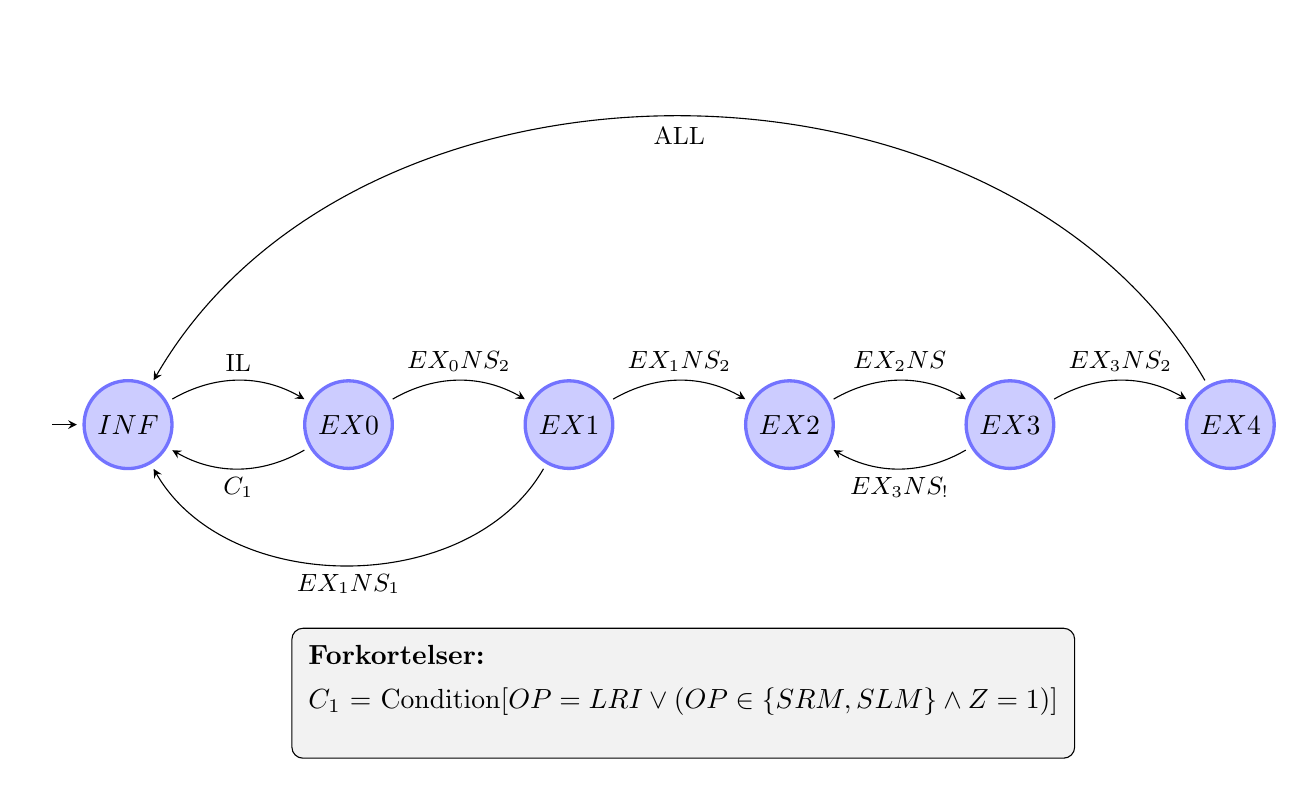
\begin{tikzpicture}
		\node[state, initial] (INF) {$INF$};
		\node[state, right of=INF] (EX0) {$EX0$};
		\node[state, right of=EX0] (EX1) {$EX1$};
		\node[state, right of=EX1] (EX2) {$EX2$};
		\node[state, right of=EX2] (EX3) {$EX3$};
		\node[state, right of=EX3] (EX4) {$EX4$};
        \node[
    draw,
    fill=gray!10,
    align=left,
    anchor=north,
    rounded corners,
    inner sep=6pt
] at ($(current bounding box.south) + (0.4,-2cm)$) {
    \textbf{Forkortelser:}\\[4pt]
    $C_1$ = Condition[$OP=LRI \lor (OP\in\{SRM,SLM\}\land Z=1)$] \\
    
};
            
		\draw
			(INF) edge[bend left] node[above]{\small IL} (EX0)
			%
			(EX0) edge[bend left] node[below]{\small $C_1$} (INF)
			(EX0) edge[bend left] node[above]{\small $EX_0NS_2$} (EX1)
			%
			(EX1) edge[bend left=60] node[below]{\small $EX_1NS_1$} (INF)
			(EX1) edge[bend left] node[above]{\small $EX_1NS_2$} (EX2)
			%
			(EX2) edge[bend left] node[above]{\small $EX_2NS$} (EX3)
			%
			(EX3) edge[bend left] node[below]{\small $EX_3NS_!$} (EX2)
			(EX3) edge[bend left] node[above]{\small $EX_3NS_2$} (EX4)
			%
			(EX4) edge[bend right=60] node[below]{\small ALL} (INF)
		;
	\end{tikzpicture}
\end{document}
